% =============================================================================
\input{resources/preamble.tex}

% ============================================================================ 
\begin{document}
\input{resources/title.tex}
\input{resources/contents.tex}

% SECTION : sections_and_references {{{
\section{Sections and References}
\label{sec:sections_and_references}
\parindent=0em

\lettrine[lines=3, findent=3pt, nindent=0pt]{T}{he} original comic book Superman
could leap tall buildings in a single bound. But then he had to come right back
down to Earth—because he didn't fly. It wasn't until the 1940s, when animators
for a new animated series decided it would be too difficult to routinely draw
him bending his knees, that it was decided that Superman could take off into the
air. Readers got to see smooth animation, and a superhero gained a new power.
\vspace{0.5cm}

% 	SUB-SECTION : tbox_references {{{
\subsection{Tbox References}
\label{ssec:tbox_references}

This is a ref to go to the tcolorboxes table \reftable{table_title}

This is a ref to go to the tcolorboxes definition \refdef{definition}

This is a ref to go to the figure in the images section \reffig{placeholder}

\subsectionend
% }}} END SUB-SECTION : tbox_references

\vspace{0.5cm}

% 	SUB-SECTION : section_refrences {{{
\subsection{Section Refrences}
\label{ssec:section_refrences}

Section \refsec{tcolorboxes}

Sub-section \refssec{tbox_references}

Sub-sub-section \refsssec{footnotes}


\subsectionend
% }}} END SUB-SECTION : section_refrences

\vspace{0.5cm}

% 		SUB-SUB-SECTION : footnotes {{{
\subsubsection{Footnotes}
\label{sssec:footnotes}

\lipsum[1-2]

This sentence has a footnote attached.\footnote{Try writing out a few
	sentences—anything at all. Now take a minute to look at how frequently each
	letter in the alphabet appears.  Chances are you'll see a lot of the letter
	"e." That's because the commonly used vowel appears in around 11 percent of
	all words in the English language, according to Oxford Dictionaries. The
	next most popular letter was "a," which appears in around 8.5 percent of all
	words. The least common letter is "q," which appears in just 0.2 percent of
	words.}


\subsubsectionend
% }}} END SUB-SUB-SECTION : footnotes

\vspace{0.5cm}

% 		SUB-SUB-SECTION : citations {{{
\subsubsection{Citations}
\label{sssec:citations}

\textbf{Types of citations aviable in natbib :}

% ENUMERATE : citations {{{

\begin{itemize}[noitemsep]

	\item \cite{einstein}
	\item \citeauthor{einstein}
	\item \citeauthor*{einstein}
	\item \citeyear{einstein}
	\item \citeyearpar{einstein}
	\item \citet{einstein} 
	\item \citet*{einstein} 
	\item \citet[chap. ~2]{einstein} 
	\item \citep{einstein} 
	\item \citep*{einstein} 
	\item \citep[see][]{einstein} 
	\item \citep[see][chap. ~2]{einstein}

\end{itemize}

% }}} END-ENUMERATE : citations

\textbf{Multiple sources , same line :}


% ENUMERATE : multiple_sources {{{

\begin{itemize}[noitemsep]

	\item \cite{einstein,lipsum}
	\item \citet{einstein,lipsum}
	\item \citep{einstein,lipsum}
	\item \citet*{einstein,lipsum}
	\item \citep*{einstein,lipsum}

\end{itemize}

% }}} END-ENUMERATE : multiple sources


\textbf{Multiple authors for the same text :}

i got too tired to read the man file , but you can do it im sure

\subsubsectionend
% }}} END SUB-SUB-SECTION : citations


\sectionend
% }}} END SECTION : sections_and_refrences

% SECTION : code {{{
\section{Code}
\label{sec:code}
\parindent=0em

\textbf{Python}
\begin{lstlisting}[language=Python]
import numpy as np

var1 = 'Hello World!' # this vairable is here just to see the string color

def incmatrix(genl1,genl2):
	m = len(genl1)
	n = len(genl2)
	M = None #to become the incidence matrix
	VT = np.zeros((n*m,1), int)  #dummy variable

	#compute the bitwise xor matrix
	M1 = bitxormatrix(genl1)
	M2 = np.triu(bitxormatrix(genl2),1) 

	for i in range(m-1):
		for j in range(i+1, m):
			[r,c] = np.where(M2 == M1[i,j])
				for k in range(len(r)):
				VT[(i)*n + r[k]] = 1;
				VT[(i)*n + c[k]] = 1;
				VT[(j)*n + r[k]] = 1;
				VT[(j)*n + c[k]] = 1;

				if M is None:
					M = np.copy(VT)
				else:
					M = np.concatenate((M, VT), 1)

				VT = np.zeros((n*m,1), int)

	return M
\end{lstlisting}

\lipsum[1]

\textbf{C++}
\begin{lstlisting}[language=C++]

#include <iostream>
#include <cmath>
using namespace std;

int main() {

	float a, b, c, x1, x2, discriminant, realPart, imaginaryPart;
	cout << "Enter coefficients a, b and c: ";
	cin >> a >> b >> c;
	discriminant = b*b - 4*a*c;

	if (discriminant > 0) {
		x1 = (-b + sqrt(discriminant)) / (2*a);
		x2 = (-b - sqrt(discriminant)) / (2*a);
		cout << "Roots are real and different." << endl;
		cout << "x1 = " << x1 << endl;
		cout << "x2 = " << x2 << endl;
	}

	else if (discriminant == 0) {
		cout << "Roots are real and same." << endl;
		x1 = (-b + sqrt(discriminant)) / (2*a);
		cout << "x1 = x2 =" << x1 << endl;
	}

	else {
		realPart = -b/(2*a);
		imaginaryPart =sqrt(-discriminant)/(2*a);
		cout << "Roots are complex and different."  << endl;
		cout << "x1 = " << realPart << "+" << imaginaryPart << "i" << endl;
		cout << "x2 = " << realPart << "-" << imaginaryPart << "i" << endl;
	}

	return 0;
}


\end{lstlisting}


\lipsum[1]


\sectionend
% }}} END SECTION : code

% SECTION : tcolorboxes {{{
\section{Tcolorboxes}
\label{sec:tcolorboxes}

\parindent=0em

% DEFINITION : definition {{{
\tcolorboxdefinition
{Definition}
{\label{def:definition}}
{

The formal statement of the meaning or significance of a word, phrase, idiom, etc., as found in dictionaries. An online dictionary resource, such as Dictionary.com, can give users direct, immediate access to the definitions of a term, allowing them to compare definitions from various dictionaries and stay up to date with an ever-expanding vocabulary.


}

% }}} END DEFINITION : definition

\lipsum[1]


% NOTE : NOTE NAME {{{

\tcolorboxnote
{

The first computer was invented in the 1940s.

}

% }}} END NOTE : note_name


\lipsum[1]


\sectionend
% }}} END SECTION : tcolorboxes

% SECTION : images_&_figures {{{
\section{Images \& Figures}
\label{sec:images_&_figures}
\parindent=0em

\lipsum[1]

% image {{{

\begin{figure}[h!]
  \includegraphics[width=\linewidth]{placeholder.jpg}
  \caption{This is a placeholder image.}
  \label{fig:placeholder}
\end{figure}

% }}}

\lipsum[1]

% page wide figure {{{

\begin{figure*}[ht]
\centering
\includegraphics[width=0.9\textwidth]{placeholder.jpg}
\caption{Wide single column figure in a twocolumn document.}
\end{figure*}

% }}}

\lipsum

% multiple images {{{

\begin{figure}[h!]
  \centering
  \begin{subfigure}[b]{0.4\linewidth}
    \includegraphics[width=\linewidth]{placeholder.jpg}
    \caption{one image.}
  \end{subfigure}
  \begin{subfigure}[b]{0.4\linewidth}
    \includegraphics[width=\linewidth]{placeholder.jpg}
    \caption{two image.}
  \end{subfigure}
  \caption{Overall image caption}
%  \label{fig:}
\end{figure}

% }}}

\sectionend
% }}} END SECTION : images_&_figures

% SECTION : tables {{{
\section{Tables}
\label{sec:tables}
\parindent=0em

	% PAGE-WIDE TABLE : new_table {{{

		\pagewidetable
		{caption}
		{ 
			p{0.25\linewidth}
			m{0.25\linewidth}
			b{0.25\linewidth} 
		}
		{
			\hline
			X & X & X\\
			X & X & X\\
			X & X & X\\

		}

	% }}} End PAGE-WIDE TABLE : new table

	% TABULARX TABLE : generic_table {{{
	
	\alternatingtabularxtable
	{0.99\linewidth}
	{llX}
	{
		cell & cell & this is the full length of a cell in \\
		cell & cell & this is the full length of a cell in \\
		cell & cell & this is the full length of a cell in \\
		cell & cell & this is the full length of a cell in \\
	
	}
	
	% }}} End TABLE : generic_table

	\lipsum[1-3]

	% XTABULAR TABLE : long_table {{{

	\alternatingxtabulartable
	{lll}
	{

	 X & X & X \\
	 X & X & X \\
	 X & X & X \\
	 X & X & X \\
	 X & X & X \\
	 X & X & X \\
	 X & X & X \\
	 X & X & X \\
	 X & X & X \\
	 X & X & X \\
	 X & X & X \\
	 X & X & X \\
	 X & X & X \\
	 X & X & X \\
	 X & X & X \\
	 X & X & X \\
	 X & X & X \\
	 X & X & X \\
	 X & X & X \\
	 X & X & X \\
	 X & X & X \\
	 X & X & X \\
	}


	% }}} End XTABULAR TABLE : long table

	\lipsum[1-4]

	\lipsum

	% TABULARX TABLE : _merged_table {{{

	\tabularxtable
	{0.99\linewidth}
	{lllX}
	{

	\hline
	\multicolumn{2}{c}{Col Merge}     & cell                         & cell \\ \midrule
	\multirow{3}{*}{ Row Merge }&
	cell & cell & cell \\ \cline{2-4}
		 &      & cell                & cell \\ \cline{3-4}
		 &      & cell                & cell \\ \midrule

	}

	% }}} End TABLE : Merged Table


\sectionend
% }}} END SECTION : tables

% SECTION : tikz {{{
\section{Tikz}
\label{sec:tikz}
\parindent=0em

\lipsum[1-2]

% tkiz two column {{{

\begin{figure}[h!]


% sigmoid  {{{

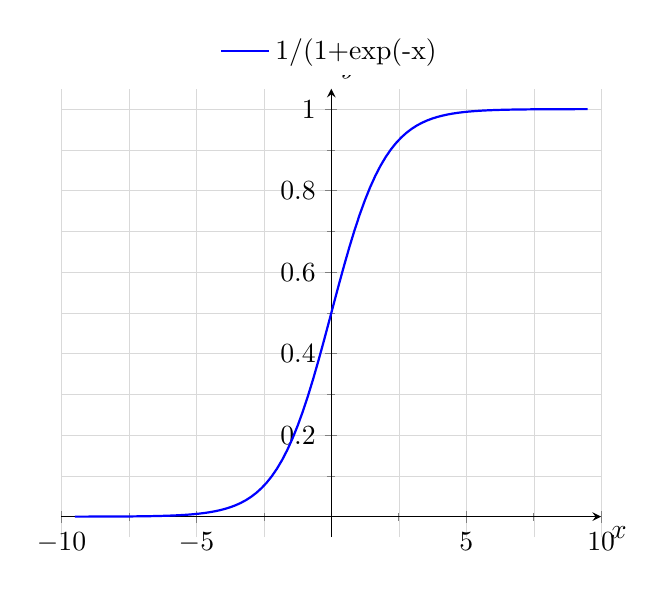
\begin{tikzpicture}
\pgfplotsset{
	every axis legend/.append style={
	at={(0.5,1.03)},
	anchor=south
},
}
\begin{axis}[
%	title          = log(x) / - log(x),
	axis x line    = middle, % x-axis post
	axis y line    = middle, % y-axis post
	minor tick num = 1,      % num axis ticks
    grid           = both,
    grid style     =
	{
		line width=.1pt,
		draw=gray!30
	},
    xmax=10,
    xmin=-10,
    ymin=-0.05,
    ymax=1.05,
	% more plot options in manual for pgfplots
	legend style =
	{
		draw = none % remove legend bounding box
	},
	xlabel       = {$x$},
	ylabel       = {$y$},
    xlabel style =
	{
		at     = {(ticklabel* cs:1)},
		anchor = north west
	},
    ylabel style=
	{
		at     = {(ticklabel* cs:1)},
		anchor = south west
	}
]

\coordinate (O) at (0,0);


\addplot [
	domain=-9.5:9.5,
	samples=100,
	thick,
	blue
]
{1/(1+exp(-x)};
\addlegendentry{1/(1+exp(-x)};

\end{axis}
\end{tikzpicture}

% }}}


\caption{This is a caption.}
\label{fig:placeholder}
\end{figure}
% }}}

\lipsum[1-2]

% tkiz two column {{{

\begin{figure}[h!]

% inv log  {{{

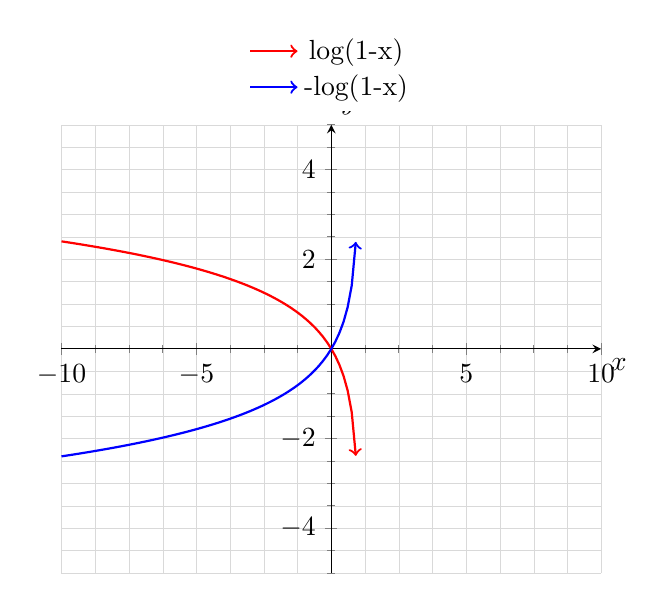
\begin{tikzpicture}

\pgfplotsset{
	every axis legend/.append style={
	at={(0.5,1.03)},
	anchor=south
},
}

\begin{axis}[
%	title          = log(x) / - log(x),
	axis x line    = middle, % x-axis post
	axis y line    = middle, % y-axis post
	minor tick num = 3,      % num axis ticks
    grid           = both,
    grid style     =
	{
		line width=.1pt,
		draw=gray!30
	},
	xmax         = 10,
	xmin         = -10,
	ymin         = -5,
	ymax         = 5,
%	legend pos = outer north east,
	legend style =
	{
		draw = none % remove legend bounding box
	},
	xlabel       = {$x$},
	ylabel       = {$y$},
    xlabel style =
	{
		at     = {(ticklabel* cs:1)},
		anchor = north west
	},
    ylabel style=
	{
		at     = {(ticklabel* cs:1)},
		anchor = south west
	},
]

\coordinate (O) at (0,0);

\addplot
[
	domain=-10:5,
	samples=100,
	thick,
	->,
	red
]
{ln(1-x)};
\addlegendentry{log(1-x)}

\addplot
[
	domain=-10:5,
	samples=100,
	thick,
	->,
	blue
]
{-ln(1-x)};
\addlegendentry{-log(1-x)}


\end{axis}
\end{tikzpicture}

%}}}



\caption{This is a caption.}
\label{fig:placeholder}
\end{figure}
% }}}

\lipsum[3-4]

% page wide tkiz figure {{{

\begin{figure*}[ht]
\centering



\tikzset{basic/.style={draw,fill=blue!50!green!20,text badly centered,minimum width=3em}}
\tikzset{input/.style={basic,circle}}
\tikzset{weights/.style={basic,rectangle,minimum width=2em}}
\tikzset{functions/.style={basic,circle,fill=blue!50!green!20}}


\newcommand{\addsymbol}{\draw[thick] (0.5em,0.5em) -- (0,0.5em) -- (0,-0.5em) --  (-0.5em,-0.5em) (0em,0.75em) -- (0em,-0.75em) (0.75em,0em) -- (-0.75em,0em);}

\begin{tikzpicture}[scale=0.75]

\foreach \h [count=\hi ] in {$x_n$,$x_2$,$x_1$,$x_0$}
{
	\node[input] (f\hi) at (0,\hi*2cm-5 cm) {\h};
}

\node[functions] (sum) at (4,0) {$\sum + bias $ };

\foreach \h [count=\hi ] in {$\theta_n$,$\theta_2$,$\theta_1$,$\theta_0$}
{
	\path (f\hi) -- node[weights] (w\hi) {\h} (sum);
	\draw[->] (f\hi) -- (w\hi);
	\draw[->] (w\hi) -- (sum);
}

% show step function symbol
\node[functions] (step) at (7,0) {};
\begin{scope}[xshift=7cm,scale=.75]
	\addsymbol
\end{scope}

\draw[->] (sum)  -- (step);
\draw[->] (step) -- ++(3,0);

% Labels
\node[above=1cm]   at (f4) {inputs};
\node[above=1cm]   at (w4) {weights};
\node[above=1cm]   at (step) {activation function};
\node[right=2.5cm] at (step) {hypothesis : $h_\theta(x)$};

\end{tikzpicture}






\caption{Wide single column figure in a twocolumn document.}
\end{figure*}

% }}}

\lipsum
\lipsum

\sectionend
% }}} END SECTION : tikz

% ----------------------------------------------------------------------------- 
\bibliography{bibliography/references} 
\end{document}
% =============================================================================
% - EOF - EOF - EOF - EOF - EOF - EOF - EOF - EOF - EOF - EOF - EOF - EOF -
% =============================================================================

